% !TEX program = lualatex
\documentclass[a4paper,11pt]{jlreq}
\usepackage{luatexja-fontspec}
\usepackage{amsmath,amssymb,mathtools,booktabs,array,graphicx}
\usepackage{tikz,pgfplots}
\usepackage[hidelinks]{hyperref}
\usepackage{xurl}
\pgfplotsset{compat=1.18}
\newcommand{\ii}{\mathrm{i}}
\newcommand{\E}{\mathbb{E}}
\newcommand{\R}{\mathbb{R}}
\newcommand{\C}{\mathbb{C}}
\DeclareMathOperator{\Rea}{Re}
\DeclareMathOperator{\Ima}{Im}
\DeclareMathOperator{\RMSE}{RMSE}
\DeclareMathOperator{\NMSE}{NMSE}
\DeclareMathOperator{\rank}{rank}
\newtheorem{proposition}{命題}
\newenvironment{proof}{\par\noindent\textbf{導出．}}{\hfill$\square$\par}
\title{tan写像の軌道情報読み出しにおける\\時間遅延特徴とTM基底の評価}
\author{長松 蒼空}
\date{2026年9月7日}
\begin{document}
\maketitle
\begin{abstract}
本研究では、$x_{t+1}=\tan(\beta x_t)$の軌道に残る時間構造を、時間遅延特徴とTakenaka--Malmquist（TM）型基底により評価する。
$\beta>1$の単一写像に対し、Cauchy不変測度の尺度に適合したCayleyモードを用いる。
周辺モード平均は0となる一方、遅延相関は$r^{k\tau}$、$r=\beta(1-\gamma^2)$となり、時間順序に生成則の差が残る。
複素モード平均の有限時間二乗誤差を相関和から導出し、独立64 seed、4パラメータ、3観測長の実験と比較する。
$\beta=1.0001$では20万時点の一次平均の理論RMSは0.22080、有効標本数は約20.51であり、経験二乗平均は理論の1.0517倍だった。
本稿は時間構造を表現する意義と有限時間精度の制約を示す。TMの回帰精度優位や同期・圧縮の成立は未検証である。
\end{abstract}
\noindent\textbf{キーワード：}tan写像、時間遅延特徴、TM基底、Cauchy不変測度、有限時間変動

\section{はじめに}
カオス軌道は不規則に見えても、時間相関には生成則に由来する構造が残りうる。
本研究の長期的な目的は、神経系の動的同期に着想を得て、カオス同期を情報圧縮へ応用できる条件を調べることである。
ただし、自由度の縮約と必要情報を保持した圧縮は同じではない。
その前段階として、単一tan写像の周辺分布と時間構造を区別し、軌道情報の読み出しを評価する。

研究質問は、(i) TM型座標をどの測度・尺度に合わせるか、
(ii) 時間遅延によって何が読み出せるか、
(iii) 臨界近傍の長い相関と有限観測長が精度にどう影響するか、の三つである。
本稿でいう読み出しは、モード平均と遅延相関の抽出・評価を指す。
未知パラメータの学習回帰や初期状態・画像の復号を実証したという意味ではない。

\section{対象写像とCauchy不変測度}
対象は
\begin{equation}
x_{t+1}=F_\beta(x_t)=\tan(\beta x_t),\qquad \beta>1
\label{eq:tan}
\end{equation}
である。極とその逆像を除く実数軌道を考える。
整数倍角写像$\gamma\tan(m\arctan(x/\gamma)+\omega)$や一般化Boole写像とは異なり、
それらの単項式共役や予測性能を本写像へ流用しない。

中心Cauchy密度を$\rho_\gamma(x)=\gamma/[\pi(x^2+\gamma^2)]$とする。
$X\sim\rho_\gamma$に対して$Y=\tan(\beta X)$の密度は、
$u=\arctan y$、$a=\beta\gamma$を用いて
\begin{align}
p_Y(y)&=\frac{a}{\pi(1+y^2)}
 \sum_{n\in\mathbb Z}\frac1{(u+n\pi)^2+a^2},\\
\sum_{n\in\mathbb Z}\frac1{(u+n\pi)^2+a^2}
&=\frac{\sinh(2a)}{a(\cosh(2a)-\cos(2u))}
\end{align}
となる。後式はCauchy核の周期化のFourier級数から得られる。
$\cos(2u)=(1-y^2)/(1+y^2)$を代入すれば
\begin{equation}
p_Y(y)=\frac{\tanh a}{\pi(y^2+\tanh^2 a)}
\end{equation}
である。したがってCauchy族の尺度は$\gamma\mapsto\tanh(\beta\gamma)$で閉じる\cite{e0}。
これは任意の初期分布や相互結合系についての閉包ではない。

$\beta>1$の正の不変尺度$\gamma\in(0,1)$は
\begin{equation}
\gamma=\tanh(\beta\gamma)
\label{eq:gamma}
\end{equation}
を満たす。以降はこの不変測度から初期化した定常過程を理論対象とする。
$\beta\downarrow1$で尺度は小さくなり、時間相関が長くなる。
有限の尺度は、実数状態の有界性を意味しない。

\section{TM型基底と遅延特徴}
\subsection{測度への適合性}
参照尺度$s>0$について
\begin{equation}
q_s(x)=\frac{x-\ii s}{x+\ii s},\qquad M_k^{(s)}(x)=q_s(x)^k
\end{equation}
と定める。本稿でいうTM型基底は共通極に対応するCayley冪であり、任意の極列を持つTM系全体は扱わない。
実数$x$では$|q_s(x)|=1$であり、モードの平均・分散は定義できる。
これは平均・分散の存在しない生のCauchy状態とは異なる。

$s=\gamma$なら$x=\gamma\tan\theta$により
\begin{equation}
\rho_\gamma(x)\,dx=\frac{d\theta}{\pi},\qquad q_\gamma(x)=-e^{2\ii\theta}
\end{equation}
となる。よって
\begin{equation}
\E[M_k\overline{M_\ell}]=\delta_{k\ell},\qquad
\E[M_k]=0\quad(k\ne0).
\end{equation}
全整数次数は$L^2(\rho_\gamma dx)$で完全な直交系となる。
正次数だけで任意の複素$L^2$関数を完全展開できるとは主張しない。
また同じCayley角度上のFourier基底とは同値であり、その間の精度優位を主張しない。

$s\ne\gamma$では$a=(\gamma-s)/(\gamma+s)$として
\begin{equation}
\E[q_s^k]=a^k,\qquad
\E[\overline{q_s^k}q_s^\ell]=a^{|\ell-k|},\quad k,\ell\ge0.
\end{equation}
円上に点が載ること自体は測度適合の証拠ではない。角度密度とGram行列を確認する必要がある。

\subsection{時間構造を読み出す相関}
$z_t=q_\gamma(x_t)$とし、正整数$k,\tau$について
\begin{equation}
C_{k,\tau}=\E[z_{t+\tau}^k\overline{z_t^k}]
=r^{k\tau},\qquad
r=\beta\,\operatorname{sech}^2(\beta\gamma)=\beta(1-\gamma^2)
\label{eq:corr}
\end{equation}
が成立する\cite{e1}。
導出には$H=q_\gamma\circ F_\beta\circ q_\gamma^{-1}$を用いる。
tan写像は上半平面を上半平面へ写し、$F_\beta(\ii\gamma)=\ii\gamma$なので、
$H$は円板の正則自己写像で$H(0)=0$、$H'(0)=r$を満たす。
$\tau$回合成$H^{\circ\tau}$の一次係数は$r^\tau$である。
$(H^{\circ\tau}(z))^k$の$k$次係数は$r^{k\tau}$であり、
円周一様測度の積分で$\overline z^{\,k}=z^{-k}$を掛けることで抽出できる。

周辺平均はどの$\beta$でも0だが、遅延相関には$\beta$の差が残る。
ただし真の尺度を用いたoracle条件であり、
未知$\beta$の推定に必要な尺度推定誤差は別途評価しなければならない。

有限窓の特徴は
\begin{align}
\widehat m_{T,k}&=\frac1T\sum_{t=1}^Tz_t^k,\\
\widehat C_{k,\tau}
&=\frac1{T-\tau}\sum_{t=1}^{T-\tau}
 z_{t+\tau}^k\overline{z_t^k}
\end{align}
の実部・虚部とする。
時間並べ替えはモード平均を保存するが遅延対を変える。
固定観測点の一様ランダム順列における異なる2点の積の条件付き期待値は
\begin{equation}
\frac{|\sum_{t=1}^T z_t^k|^2-T}{T(T-1)}
\end{equation}
であり、有限標本の並べ替え相関を必ず0とはみなせない。

\section{有限時間の推定精度}
定常初期化でも単一軌道の時間平均は一般に0にならない。
二乗を展開し、距離$h$の対が$T-h$個あることを用いると
\begin{equation}
V(T,k)=\E[|\widehat m_{T,k}|^2]
=\frac{T+2\sum_{h=1}^{T-1}(T-h)r^{kh}}{T^2}.
\label{eq:variance}
\end{equation}
正次数の非共役積の平均は0であり、実部・虚部の分散はいずれも$V/2$、共分散は0となる。
これは複素平均の正規分布性を意味しない。

十分長い$T$では
\begin{equation}
V(T,k)\sim\frac{1+r^k}{1-r^k}\frac1T,\qquad N_{\mathrm{eff}}=\frac1{V(T,k)}
\end{equation}
となる。$N_{\mathrm{eff}}$は単位二乗モードの平均精度に関する有効標本数であり、
他の統計量や遅延相関推定器へそのまま適用できる量ではない。
臨界近傍では$r$が1に近いため、独立標本を仮定した$1/T$の二乗誤差は不適切である。

\section{数値実験と結果}
\subsection{設計}
主結果は保存済みの有限時間確認実験\cite{confirmation}であり、この改稿では軌道を再生成していない。
$\beta=1.0001,1.01,1.1,2.0$の各64独立seed、
$T=50{,}000,200{,}000,1{,}000{,}000$、
$k=1,2,4,8$を事前に固定した。
不変Cauchy初期値からburn-inなしで$x_1$以降を観測した。
観測長間は同じ軌道の先頭区間を使うため独立ではない。
相関は$k=1,4$、$\tau=1,64,1024,4096$に固定した。

float64、Numbaの標準tan、fastmathなしで実行し、クリップ・seed交換を行わない。
理論式は明示和・Toeplitz行列・円板積分で先に照合した。
区間は独立seed単位のStudent-$t$近似95\%区間であり、
多重比較の一括採択や厳密な被覆保証には使わない。

\subsection{臨界近傍の有限時間変動}
\begin{table}[htbp]\centering\small
\caption{$\beta=1.0001$、$k=1$の64 seed平均。半幅は近似95\%区間。}\label{tab:main}
\begin{tabular}{rrrrr}\toprule
$T$ & 理論$V$ & 経験二乗平均 & 区間半幅 & 経験/理論\\\midrule
50,000&0.1800041&0.1827277&0.0366150&1.0151\\
200,000&0.0487510&0.0512718&0.0117003&1.0517\\
1,000,000&0.0099502&0.0097589&0.0024033&0.9808\\\bottomrule
\end{tabular}
\end{table}
表\ref{tab:main}では全3観測長で経験二乗平均が有限長の理論値と対応する。
20万時点の理論RMSは0.22080、有効標本数は20.51、
100万時点ではそれぞれ0.09975、100.50となる。
20万時点を20万独立標本と同じ精度で扱うことはできない。

先行する代表軌道解析では同じ$\beta$、20万時点の一次平均が
$0.00300644-0.29182229\ii$だった\cite{e1}。
この偏りだけで理論不一致とは判定できない。
追試は長い相関による有限時間変動という説明を支持するが、
前回の特定軌道の原因を一意に証明したものではない。

\begin{figure}[p]\centering
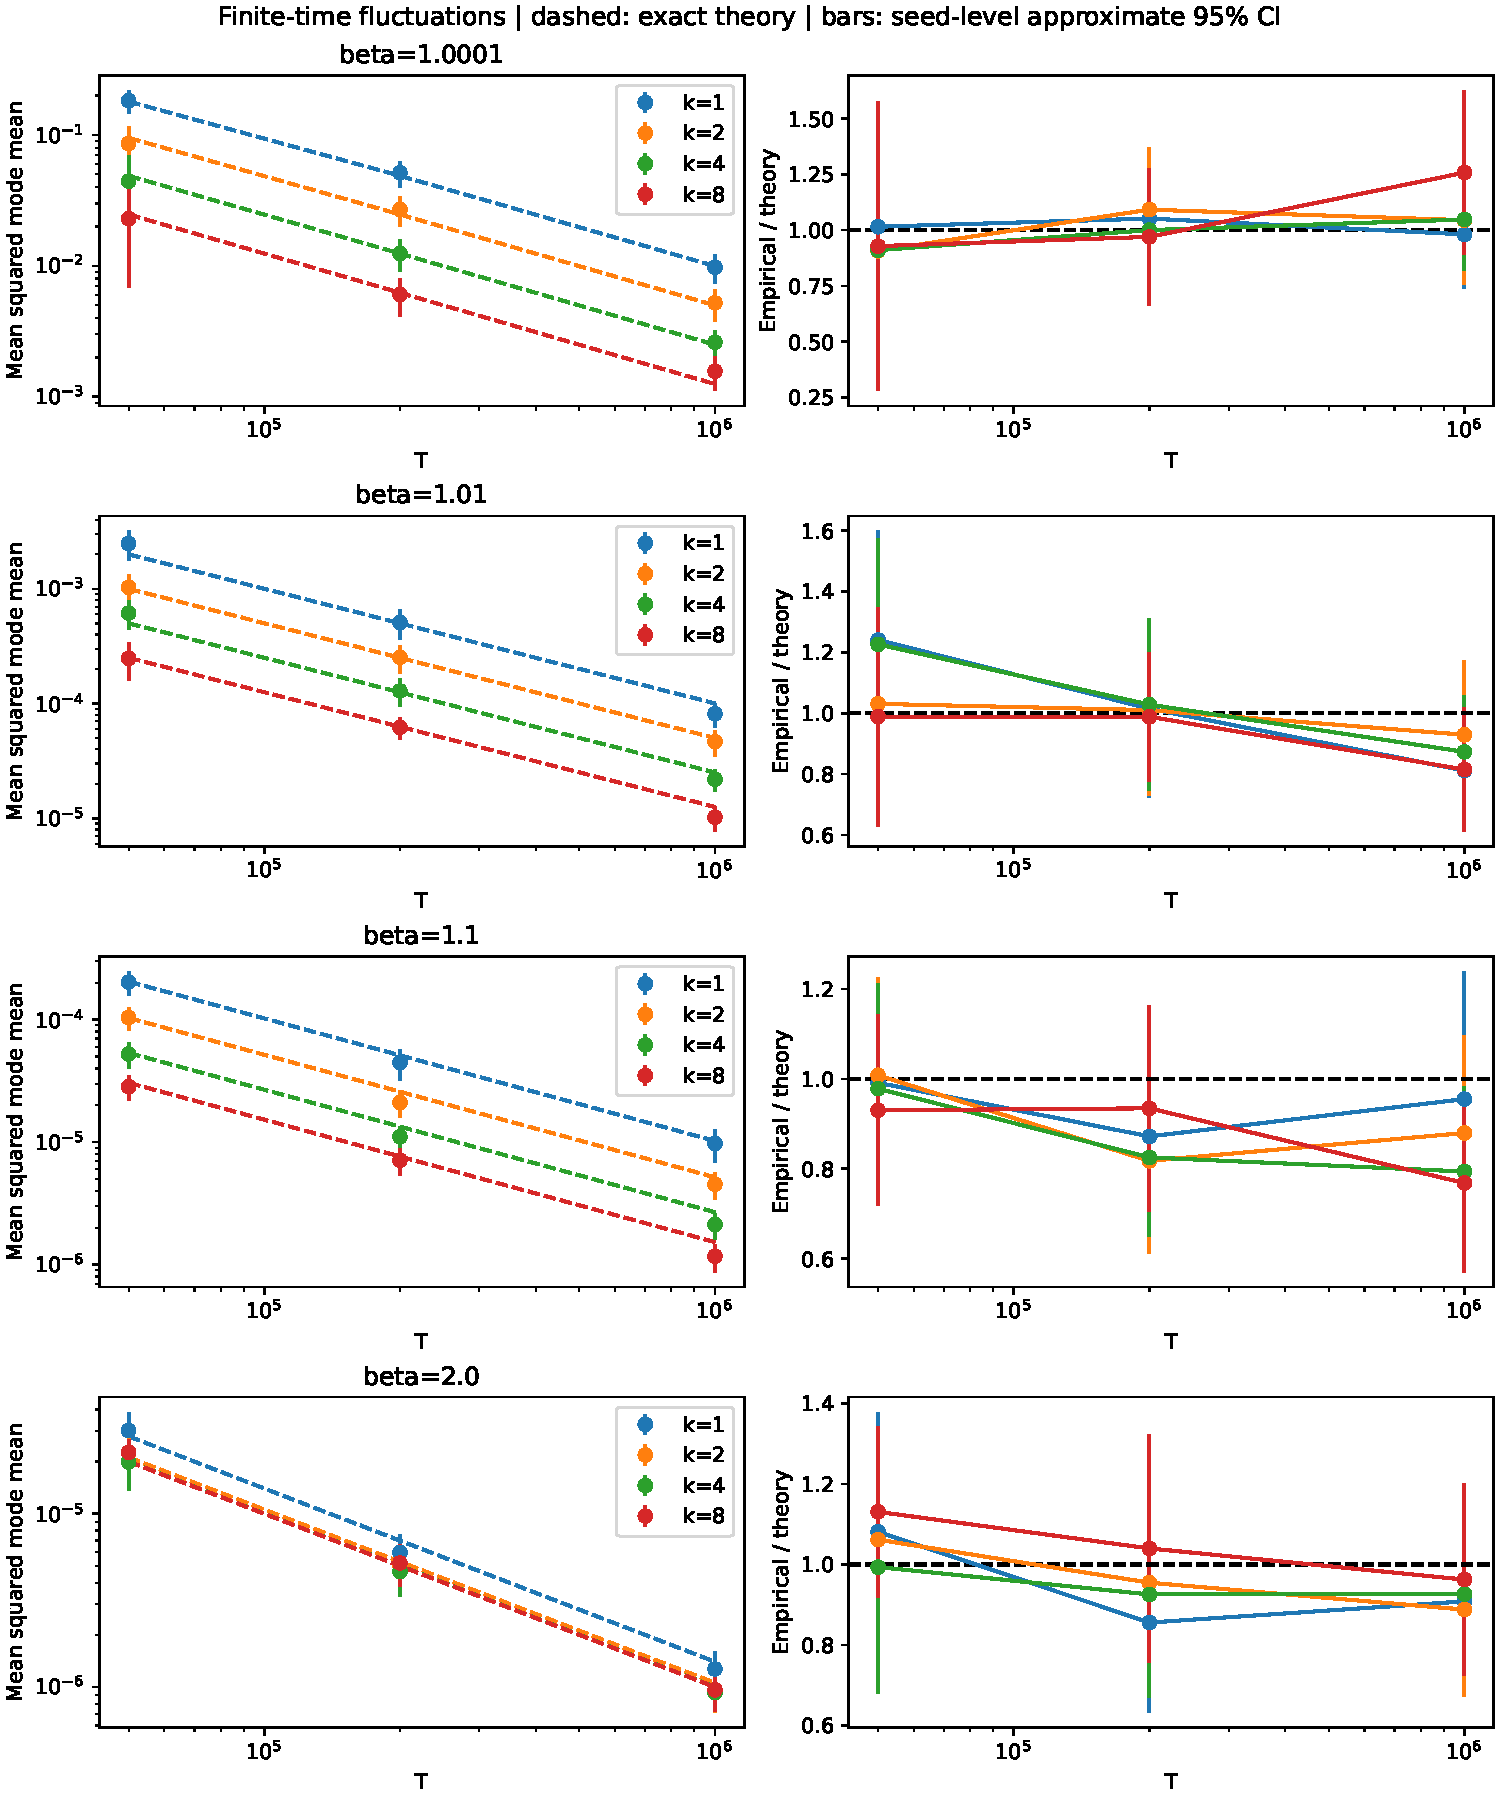
\includegraphics[width=\linewidth,height=.77\textheight,keepaspectratio]{../../projects/chaos-sync-thesis/experiments/runs/20260907_E1_tangent-finite-time-confirmation/artifacts/fig2_finite_time_scaling.pdf}
\caption{モード平均二乗の観測長依存と有限長理論。元データは確認実験のsummary.csv。
区間は64 seed単位の近似95\%区間。観測長・モード間には依存がある。}
\end{figure}

\subsection{条件差と遅延相関}
48条件中46条件で近似95\%区間が理論を含んだ。
含まなかった$\beta=1.1$、100万時点の$k=4,8$は、
経験/理論比が0.79388、0.76828だった。
これを全仮説採択とも、2条件だけによる理論反証とも扱わない。

100万時点のseed平均相関の最大複素誤差は0.0088782で、
$\beta=1.0001$、$k=4$、$\tau=4096$に生じた。
経験値は$0.0363667+0.0087696\ii$、理論値は0.0377513だった。
代表seed解析とはモード・観測長・seed数が異なるため、単純な改善率は計算しない。

\begin{figure}[p]\centering
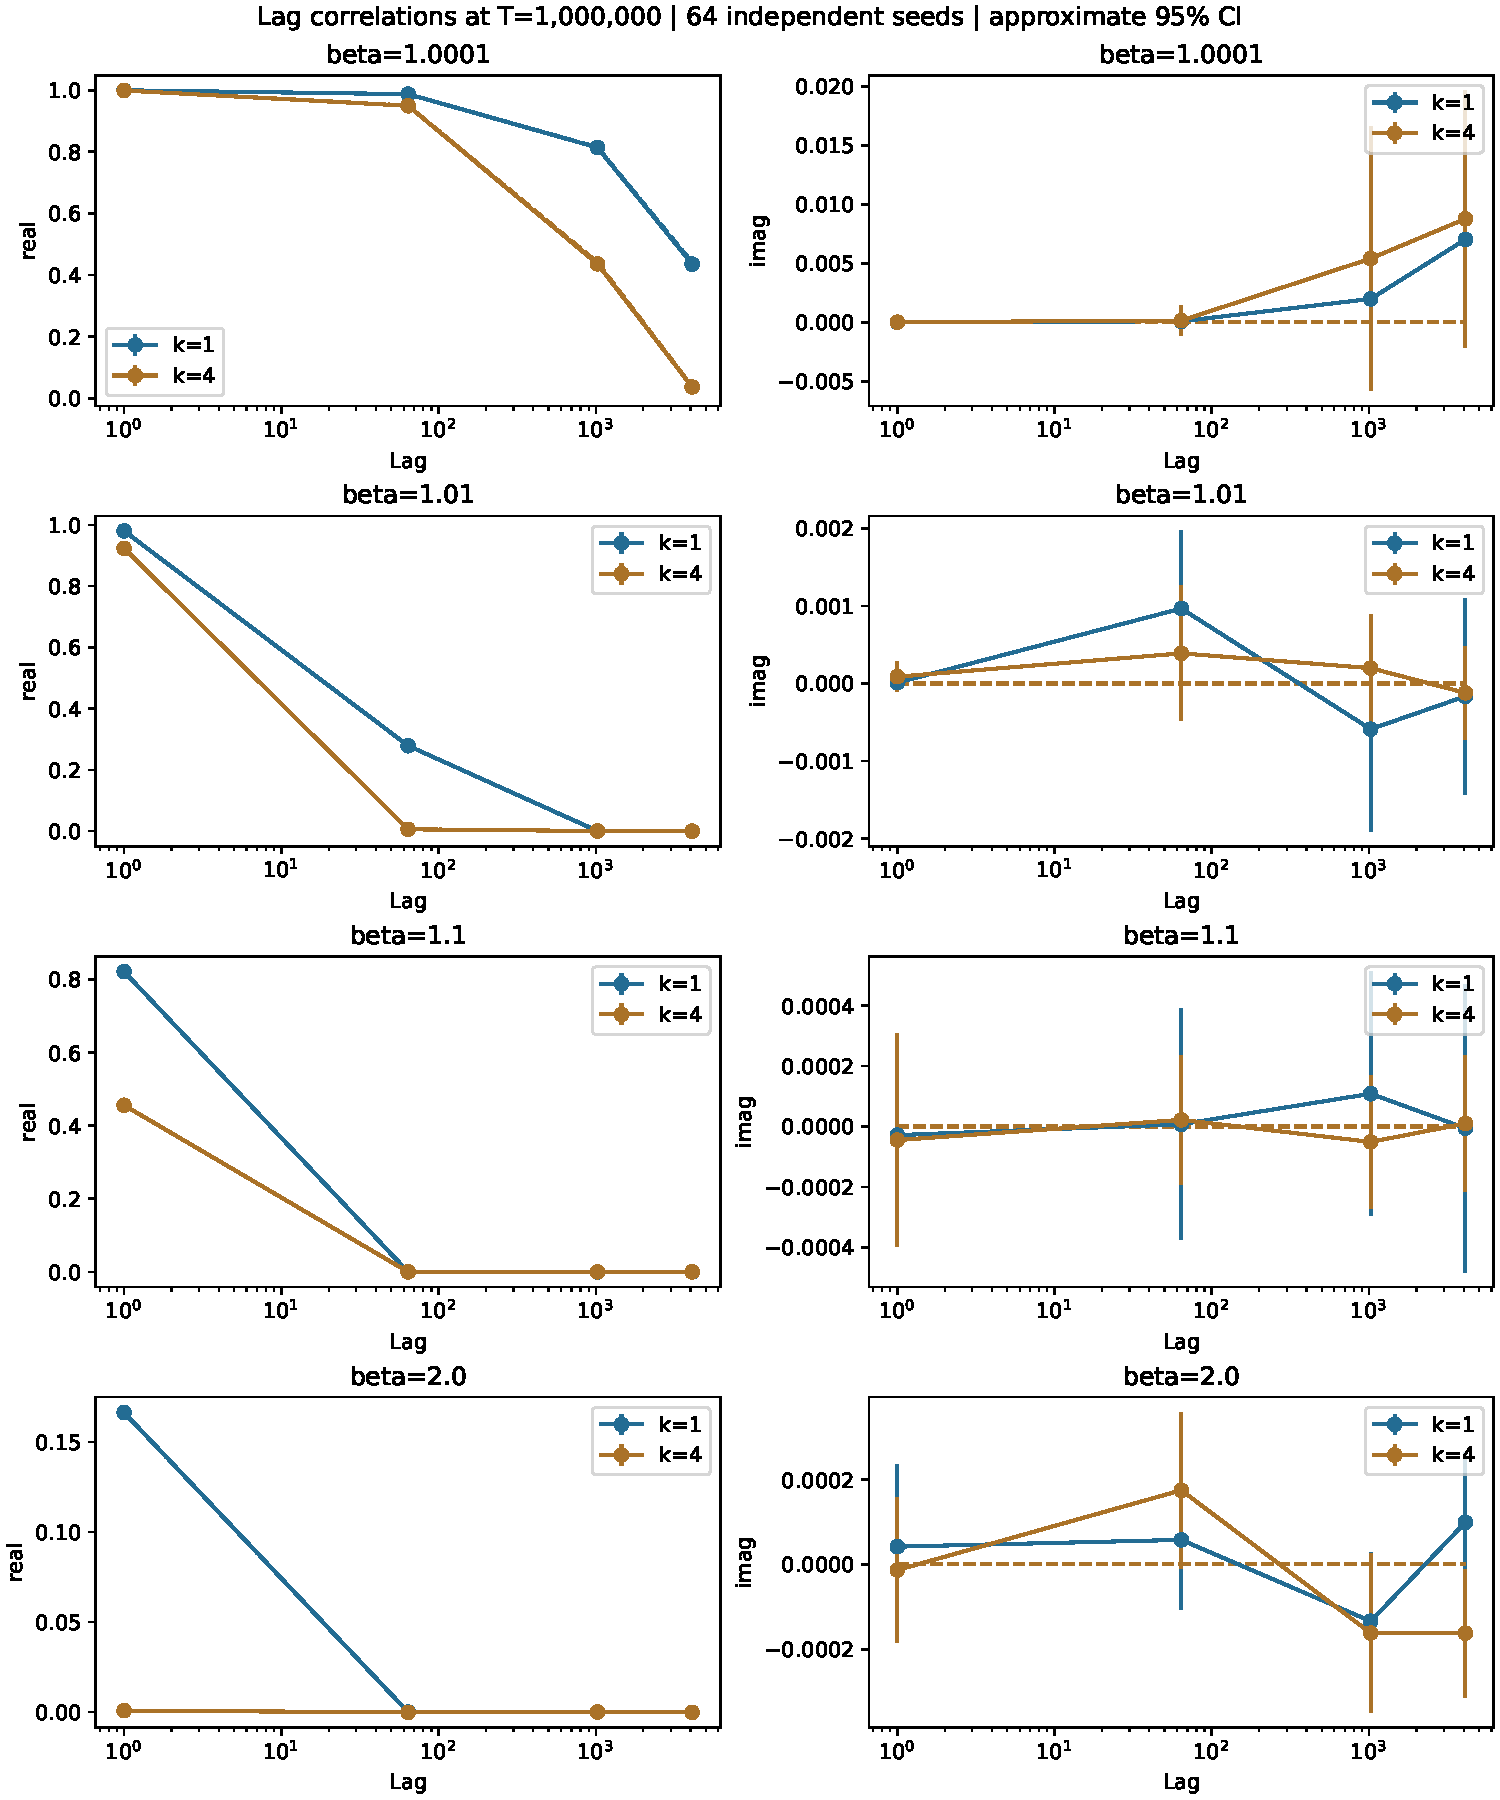
\includegraphics[width=\linewidth,height=.77\textheight,keepaspectratio]{../../projects/chaos-sync-thesis/experiments/runs/20260907_E1_tangent-finite-time-confirmation/artifacts/fig4_correlations.pdf}
\caption{100万時点、$k=1,4$の相関実部・虚部。元データはcorrelations.csv。
点と区間は64 seedの集計、破線は$r^{k\tau}$。}
\end{figure}

\subsection{数値整合性と不一致}
256軌道・2.56億更新でゼロ出現・非有限値は0件、
単位円誤差最大は$2.22045\times10^{-16}$だった。
理論52項目の最大誤差は$1.6654\times10^{-15}$である。
これらは数値整合性の証拠であり、回帰性能の証拠ではない。

先行E0の一ステップCauchy検定はfloat64の210条件中209条件が基準を満たした\cite{e0}。
超過1条件は$\beta=1$、初期尺度1で、高精度の同一標本診断でも残った。
今回の$\beta>1$の主評価とは区別し、全条件通過とは記述しない。
先行float32実験の有限精度反復も、厳密実数理論とデジタル軌道の違いとして残る。

\section{考察と今後の課題}
TM型基底はCauchy測度に適合した有界な座標として時間構造を記述できる。
周辺平均では消える生成則の差が遅延相関に残るため、
時間順序を保つ特徴設計には理論的根拠がある。
一方、臨界近傍の長い相関は有限窓の平均のばらつきを増す。
座標の測度適合性と推定値の安定性は別の評価軸である。

本稿は真の尺度を用いた評価である。次の未知パラメータ回帰では、
観測からの推定尺度とoracle尺度を分け、独立seedと未学習$\beta$による分割を事前に固定する必要がある。
TM遅延、遅延なしTM、実数時系列Fourier、Cayley時系列Fourier、並べ替え対照を、
同一特徴次元・同一回帰器で比較することが課題となる。
一般化Boole写像の既存回帰結果は別系列であり、tan写像の優劣の証拠にはしない。

観測ノイズ、欠損、同期、量子化後の符号長と復号歪みは未評価である。
相互結合へ進むには、同期多様体・不変測度・横方向安定性を別に導出しなければならない。
今回の結果から圧縮、画像復号、脳の省エネルギー性の説明が成立したとは結論しない。

\section{結論}
tan写像$\tan(\beta x)$について、TM型基底の測度適合性、遅延相関、有限時間精度を評価した。
尺度適合した周辺平均は0だが遅延相関は$r^{k\tau}$となり、生成則の差が時間構造に残る。
64 seed追試では臨界近傍の平均二乗変動が厳密な相関和と対応した。
本発表の成果は時間遅延特徴の理論的意義と有限時間推定の制約を示したことである。
TMの他手法への予測精度優位と圧縮・復号の実証は別の評価として残る。

\appendix
\section{再現資料}
各実験の正本は研究プロジェクト内の\path{experiments/runs/}以下にある。
主表は確認実験の\path{artifacts/summary.csv}、相関は\path{artifacts/correlations.csv}、
seed別モード平均は\path{artifacts/moments.csv}に対応する。
条件・導出・結果はREADME、事前登録本文は\path{theory.json}、
環境は\path{environment.json}に保存されている。
入口は\path{finite_time.py}で、図と集計は保存データから再生成できる。
本文のRMSは漸近近似でなく式\eqref{eq:variance}の有限和による。
本改稿では既存保存値と図を使用し、新しい科学実験は実施していない。

\begin{thebibliography}{9}
\bibitem{e0} 長松蒼空，「E0: tan(beta x) のコーシー保存・臨界挙動」，未公刊実験記録，2026年9月6日．
\path{20260906_E0_tangent-cauchy/README.md}．
\bibitem{e1} 長松蒼空，「tan写像のTM複素平面・時間構造の評価」，未公刊実験記録，2026年9月6日．
\path{20260906_E1_tangent-tm-complex-plane/README.md}．
\bibitem{confirmation} 長松蒼空，「E1追試：TM時間平均の有限時間変動」，未公刊実験記録，2026年9月7日．
\path{20260907_E1_tangent-finite-time-confirmation/README.md}．
\end{thebibliography}
\end{document}